
\chapter{Cadenas }

\label{strings}

\section{Un tipo de dato compuesto}

\index{tipo de dato compuesto} \index{tipo de dato!compuesto}

Hasta aquí hemos visto tres tipos de datos: \texttt{int}, \texttt{float}
y \texttt{string}. Las cadenas son cualitativamente diferentes de
los otros dos tipos porque están compuestas de piezas más pequeñas—los
caracteres.

\index{carácter}

Los tipos que comprenden piezas más pequeñas se denominan \textbf{tipos
de datos compuestos}. Dependiendo de lo que hagamos podemos tratar
un tipo compuesto como unidad o podemos acceder a sus partes. Esta
ambigüedad es provechosa.

\index{operador corchete} \index{operador!corchete}

El operador corchete selecciona un carácter de una cadena.

\inputencoding{latin9}\begin{lstlisting}
>>> fruta = "banano"
>>> letra = fruta[1]
>>> print(letra)	
\end{lstlisting}
\inputencoding{utf8}
La expresión \texttt{fruta{[}1{]}} selecciona el carácter número 1
de \texttt{fruta}. La variable \texttt{letra} se refiere al resultado.
Cuando desplegamos \texttt{letra}, obtenemos una pequeña sorpresa:
\begin{verbatim}
a
\end{verbatim}
La primera letra de ``banano'' no es \texttt{a}. ¡A menos que usted
sea un científico de la computación! Por razones perversas, los científicos
de la computación empiezan a contar desde cero. La letra número 0
de \texttt{``banano''} es \texttt{b}. La letra 1 es a, y la letra
2 es n.

Si usted desea la primera letra de una cadena se pone 0, o cualquier
expresión con el valor 0, dentro de los corchetes:\inputencoding{latin9}
\begin{lstlisting}
>>> letra = fruta[0]
>>> print(letra)
b
\end{lstlisting}
\inputencoding{utf8}
La expresión en corchetes se denomina \textbf{índice}. Un índice especifica
un miembro de un conjunto ordenado, en este caso el conjunto de caracteres
de la cadena. El índice {\em indica} cual elemento desea usted,
por eso se llama así. Puede ser cualquier expresión entera.

\index{índice}

\section{Longitud}

\index{cadena!longitud} \index{error de tiempo de ejecución}

La función \texttt{len} retorna el número de caracteres en una cadena:

\inputencoding{latin9}\begin{lstlisting}
>>> fruta = "banano"
>>> len(fruta)
6
\end{lstlisting}
\inputencoding{utf8} Para acceder a la última letra de una cadena usted podría caer en
algo como esto:\inputencoding{latin9}
\begin{lstlisting}
longitud = len(fruta)
ultima = fruta[longitud]       # ERROR!
\end{lstlisting}
\inputencoding{utf8}
Y no funcionará. Causa un error en tiempo de ejecución, \texttt{IndexError: string
index out of range}. La razón yace en que no hay una letra 6 en ``banano''.
Como empezamos a contar desde cero, las seis letras se numeran de
0 a 5. En general, para obtener la última letra, tenemos que restar
1 a la \texttt{longitud}:

\index{error en tiempo de ejecución}

\inputencoding{latin9}\begin{lstlisting}
longitud = len(fruta)
ultima = fruta[longitud-1]
\end{lstlisting}
\inputencoding{utf8}
Alternativamente, podemos usar índices negativos, que cuentan hacia
atrás desde el fin de la cadena. La expresión \texttt{fruta{[}-1{]}}
retorna la última letra \texttt{fruta{[}-2{]}} retorna la penúltima,
y así sucesivamente.

\index{índice!negativo}

\section{Recorridos en cadenas y el ciclo \texttt{for}}

\label{for} 

\index{recorridos} \index{ciclo!recorrido} \index{ciclo for} \index{ciclo!ciclo for}

Muchos cálculos implican procesar una cadena carácter por carácter.
A menudo empiezan al inicio, seleccionan cada carácter en cada paso,
le hacen algo y continúan hasta el final. Este patrón de procesamiento
se denomina \textbf{recorrido}. Hay una forma de realizarlo con la
sentencia \texttt{while}:\inputencoding{latin9}
\begin{lstlisting}
indice = 0
while indice < len(fruta):
  letra = fruta[indice]
  print(letra)
  indice = indice + 1
\end{lstlisting}
\inputencoding{utf8}
Este ciclo recorre la cadena y despliega cada letra en una línea independiente.
La condición del ciclo es \texttt{indice < len(fruta)}, así que cuando
\texttt{indice} se hace igual a la longitud de la cadena, la condición
es falsa, y el cuerpo del ciclo no se ejecuta. El último carácter
accedido es el que tiene el índice \texttt{len(fruta)-1}, es decir,
el último.

Usar un índice para recorrer un conjunto de valores es tan común que
Python tiene una sintaxis alternativa más simple—el ciclo \texttt{for}
:

\inputencoding{latin9}\begin{lstlisting}
for caracter in fruta:
   print(caracter)
\end{lstlisting}
\inputencoding{utf8}
Cada vez que el ciclo itera, el próximo carácter en la cadena se asigna
a la variable \texttt{caracter}. El ciclo continúa hasta que no quedan
más caracteres.

\index{concatenación} \index{lexicográfico} \index{McCloskey, Robert}
\index{Make Way for Ducklings@{\em Make Way for Ducklings}}

El siguiente ejemplo muestra cómo usar la concatenación y un ciclo
\texttt{for} para generar una serie en orden lexicográfico. Lexicográfico
se refiere a una lista en la que los elementos aparecen en orden alfabético.
Por ejemplo, en el libro {\em Make Way for Ducklings} de Robert
McCloskey, los nombres de los patos son Jack, Kack, Lack, Mack, Nack,
Ouack, Pack, and Quack. Este ciclo los despliega en orden:\inputencoding{latin9}
\begin{lstlisting}
prefijos = "JKLMNOPQ"
sufijo = "ack"

for letra in prefijos:
  print(letra + sufijo)
\end{lstlisting}
\inputencoding{utf8}
La salida de este programa es:\inputencoding{latin9}
\begin{lstlisting}
Jack
Kack
Lack
Mack
Nack
Oack
Pack
Qack
\end{lstlisting}
\inputencoding{utf8}
Por supuesto que hay un error, ya que ``Ouack'' y ``Quack'' no
están bien deletreados.

\section{Segmentos de cadenas }

\label{slice} \index{segmento} \index{cadena!segmento}

Una porción de una cadena de caracteres se denomina \textbf{segmento}.
Seleccionar un segmento es similar a seleccionar un carácter:\inputencoding{latin9}
\begin{lstlisting}
>>> s = "Pedro, Pablo, y Maria"
>>> print(s[0:5])
Pedro
>>> print(s[7:12])
Pablo
>>> print(s[16:21])
Maria
\end{lstlisting}
\inputencoding{utf8}
El operador \texttt{{[}n:m{]}} retorna la parte de la cadena que va
desde el carácter n hasta el m, incluyendo el primero y excluyendo
el último. Este comportamiento es contraintuitivo, tiene más sentido
si se imagina que los índices van {\em antes} de los caracteres,
como en el siguiente diagrama:

\beforefig \centerline{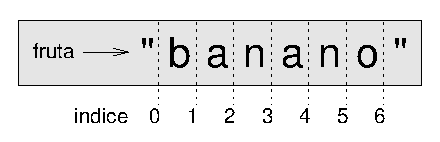
\includegraphics{illustrations/banana}}
\afterfig

Si usted omite el primer índice (antes de los puntos seguidos), el
segmento comienza en el inicio de la cadena. Si se omite el segundo
índice, el segmento va hasta el final. Entonces:\inputencoding{latin9}
\begin{lstlisting}
>>> fruta  = "banano"
>>> fruta[:3]
'ban'
>>> f[3:]
'ano'
\end{lstlisting}
\inputencoding{utf8} ¿Que cree que significa \texttt{s{[}:{]}}?

\section{Comparación de cadenas}

\index{comparación de cadenas} \index{comparación!de cadenas}

El operador de comparación funciona con cadenas. Para ver si dos cadenas
son iguales:\inputencoding{latin9}
\begin{lstlisting}
if palabra == "banana":
  print("No hay bananas!")
\end{lstlisting}
\inputencoding{utf8}Las otras operaciones de comparación son útiles para poner las palabras
en orden alfabético:\inputencoding{latin9}
\begin{lstlisting}
if palabra < "banana":
  print("Su palabra," + palabra + ", va antes que banana.")
elif palabra > "banana":
  print("Su palabra," + palabra + ", va despu�s de banana.")
else:
  print("No hay banana!")
\end{lstlisting}
\inputencoding{utf8}
Sin embargo, usted debe ser consciente de que Python no maneja las
letras minúsculas y mayúsculas de la misma forma en que lo hace la
gente. Todas las letras mayúsculas vienen antes de las minúsculas.
Si palabra vale ``Zebra'' la salida sería:
\begin{verbatim}
Su palabra, Zebra, va antes que banana.
\end{verbatim}
Este problema se resuelve usualmente convirtiendo las cadenas a un
formato común, todas en minúsculas por ejemplo, antes de hacer la
comparación. Un problema más difícil es lograr que el programa reconozca
que una zebra no es una fruta.

\section{Las cadenas son inmutables}

\index{mutable} \index{cadena inmutable} \index{cadena!inmutable}

Uno puede caer en la trampa de usar el operador \texttt{{[}{]}} al
lado izquierdo de una asignación con la intención de modificar un
carácter en una cadena. Por ejemplo:\inputencoding{latin9}
\begin{lstlisting}
saludo = "Hola mundo"
saludo[0] = 'J'            # ERROR!
print(saludo)
\end{lstlisting}
\inputencoding{utf8} En lugar de desplegar \texttt{Jola mundo!}, se produce un error en
tiempo de ejecución \texttt{TypeError: object doesn't support item
assignment}.

\index{error en tiempo de ejecución}

Las cadenas son \textbf{inmutables}, lo que quiere decir que no se
puede cambiar una cadena existente. Lo máximo que se puede hacer es
crear otra cadena que cambia un poco a la original:\inputencoding{latin9}
\begin{lstlisting}
saludo = "Hola mundo!"
nuevoSaludo = 'J' + saludo[1:]
print(nuevoSaludo)
\end{lstlisting}
\inputencoding{utf8}
La solución consiste en concatenar la primera nueva letra con un segmento
de \texttt{saludo}. Esto no tiene efecto sobre la primera cadena,
usted puede chequearlo.

\index{concatenación}

\section{Una función \texttt{buscar} }

\label{find} \index{recorrido} \index{recorrido eureka} \index{patrón}
\index{patrón computacional}

¿Qué hace la siguiente función?

\inputencoding{latin9}\begin{lstlisting}
def buscar(cad, c):
  indice = 0
  while indice < len(cad):
    if cad[indice] == c:
      return indice
    indice = indice + 1
  return -1
\end{lstlisting}
\inputencoding{utf8} De cierta manera \texttt{buscar} es el opuesto del operador \texttt{{[}{]}}.
En vez de tomar un índice y extraer el carácter correspondiente, toma
un carácter y encuentra el índice donde éste se encuentra. Si no se
encuentra el carácter en la cadena, la función retorna \texttt{-1}.

Este es el primer ejemplo de una sentencia \texttt{return} dentro
de un ciclo. Si se cumple que \texttt{cadena{[}indice{]} == c}, la
función retorna inmediatamente, rompiendo el ciclo prematuramente.

Si el carácter no está en la cadena, el programa completa todo el
ciclo y retorna \texttt{-1}.

Este patrón computacional se denomina recorrido ``eureka'', ya que
tan pronto encontremos lo que buscamos, gritamos ``Eureka!'' y dejamos
de buscar.

\section{Iterando y contando}

\label{counter} \index{contador} \index{patrón}

El siguiente programa cuenta el número de veces que la letra \texttt{a}
aparece en una cadena:\inputencoding{latin9}
\begin{lstlisting}
fruta = "banano"
cont = 0
for car in fruta:
  if car == 'a':
    cont = cont + 1
print(cont)
\end{lstlisting}
\inputencoding{utf8} Este programa demuestra otro patrón computacional denominado \textbf{contador}.
La variable \texttt{cont} se inicializa a 0 y se incrementa cada vez
que se encuentre una \texttt{a}. ( \textbf{incrementar} es añadir
uno; es el opuesto de \textbf{decrementar}, y no tienen nada que ver
con ``excremento,'' que es un sustantivo.) Cuando el ciclo finaliza,
\texttt{cont} contiene el resultado—el número total de \texttt{a}'s.

\section{Algunos métodos de las cadenas}

\index{cadenas!métodos} \index{método} \index{método!invocación}
\index{métodos!cadenas} \index{métodos sobre cadenas} \index{invocar métodos}

Un \textbf{método} es similar a una función, acepta parámetros y devuelve
un valor, pero la sintaxis es diferente. Por ejemplo, las cadenas
tienen un método denominado \texttt{find} que hace lo mismo que buscar.
Para llamarlo tenemos que especificar la cadena, o la variable que
contiene la cadena, usando la notación punto, en la que el método
se escribe después del punto. La llamada a un método también se denomina
\textbf{invocación}; en este caso, diríamos que estamos invocando
\texttt{find} sobre la cadena \texttt{fruta}.

\inputencoding{latin9}\begin{lstlisting}
>>> fruta = "banano"
>>> ind = fruta.find("a")
>>> print(ind)
1
\end{lstlisting}
\inputencoding{utf8}
El método \texttt{find} es más general que buscar, también puede buscar
subcadenas, no solo caracteres:\inputencoding{latin9}
\begin{lstlisting}
>>> "banano".find("na")
2
\end{lstlisting}
\inputencoding{utf8}
También tiene un argumento adicional que especifica el índice desde
el que debe empezar la búsqueda:\inputencoding{latin9}
\begin{lstlisting}
>>> "banana".find("na",3) 
4
\end{lstlisting}
\inputencoding{utf8}
Igualmente, puede tomar dos argumentos adicionales que especifican
un rango de índices:\inputencoding{latin9}
\begin{lstlisting}
>>> "bob".find("b",1,2) 
-1
\end{lstlisting}
\inputencoding{utf8}
Aquí la búsqueda falló porque la letra {\em b} no está en en el
rango de índices de \texttt{1} a \texttt{2} (recuerde que no se incluye
el último índice, el \texttt{2}).

\section{El módulo \texttt{string y} clasificación de caracteres}

\index{módulo} \index{módulo string}

\label{in} \index{clasificación de caracteres} \index{clasificación!de caracteres}
\index{mayúsculas} \index{minúsculas} \index{espacios en blanco}

Con frecuencia es útil examinar un carácter y decidir si está en mayúsculas
o en minúsculas, o si es un dígito. El módulo \texttt{string} proporciona
varias constantes que sirven para lograr estos objetivos.

La cadena \texttt{string.lowercase} contiene todas las letras que
el sistema considera como minúsculas. Igualmente, \texttt{string.uppercase}
contiene todas las letras mayúsculas. Intente lo siguiente y vea por
sí mismo:\inputencoding{latin9}
\begin{lstlisting}
>>> import string
>>> print(string.ascii_lowercase)
>>> print(string.ascii_uppercase)
>>> print(string.digits)
\end{lstlisting}
\inputencoding{utf8}Podemos usar estas constantes y el método \texttt{find} para clasificar
los caracteres. Por ejemplo, si \texttt{c.find(lowercase)} retorna
un valor distinto de \texttt{-1}, entonces \texttt{c} debe ser una
letra minúscula:\inputencoding{latin9}
\begin{lstlisting}
import string

def esMinuscula(c):
  return string.ascii_lowercase.find(c) != -1
\end{lstlisting}
\inputencoding{utf8}
Otra alternativa la da el operador \texttt{in} que determina si un
carácter aparece en una cadena:\inputencoding{latin9}
\begin{lstlisting}
def esMinuscula(c):
  return c in string.ascii_lowercase
\end{lstlisting}
\inputencoding{utf8} Y otra alternativa más, con el operador de comparación:\inputencoding{latin9}
\begin{lstlisting}
def esMinuscula(c):
  return 'a' <= c <= 'z'
\end{lstlisting}
\inputencoding{utf8}
Si \texttt{c} está entre {\em a} y {\em z}, debe ser una letra
minúscula.

Otra constante definida en el módulo \texttt{string} puede sorprenderlo
cuando la imprima:\inputencoding{latin9}
\begin{lstlisting}
>>> print(string.whitespace)
\end{lstlisting}
\inputencoding{utf8}
Un carácter de los que pertenecen a \textbf{whitespace} mueve el cursor
sin imprimir nada. Crean un espacio en blanco que se puede evidenciar
entre caracteres. La constante \texttt{string.whitespace} contiene
todos los caracteres que representan espacios en blanco: espacio,
tab (\verb+\t+), y nueva línea (\verb+\n+).

\index{módulo string} \index{módulo!string}

Hay otras funciones útiles en el módulo string, pero este libro no
es un manual de referencia. Para esto usted puede consultar la referencia
de las bibliotecas de Python ({\em Python Library Reference}).
Además, hay un gran cúmulo de documentación en el sitio web de Python
\texttt{www.python.org}.

\index{Python Library Reference@{\em Python Library Reference}}

\section{Glosario}
\begin{description}
\item [{Tipo de dato compuesto:}] un tipo de dato en el que los valores
están compuestos por componentes o elementos, que, a su vez, son valores.
\item [{Recorrido:}] iteración sobre todos los elementos de un conjunto
ejecutando una operación similar en cada uno.
\item [{Índice:}] variable o valor que se usa para seleccionar un miembro
de un conjunto ordenado, tal como los caracteres de una cadena. También
se puede usar el término \texttt{posición} como sinónimo de índice.
\item [{Segmento:}] parte de una cadena, especificada por un rango de índices.
\item [{Mutable:}] un tipo de dato compuesto a cuyos elementos pueden asignarseles
nuevos valores.
\item [{Contador:}] una variable que se usa para contar algo, usualmente
se inicializa en cero y se incrementa posteriormente dentro de un
ciclo.
\item [{Incrementar:}] agregar uno al valor de una variable
\item [{Decrementar:}] restar uno al valor de una variable
\item [{Espacio en blanco:}] cualquiera de los caracteres que mueven el
cursor sin imprimir nada visible. La constante \texttt{string.whitespace}
contiene todos los caracteres que representan espacios en blanco.

\index{tipo de dato compuesto} \index{recorrido} \index{índice}
\index{segmento} \index{mutable} \index{contador} \index{incrementar}
\index{decrementar} \index{espacio en blanco}
\end{description}

\section{Ejercicios}

Para cada función, agregue chequeo de tipos y pruebas unitarias.
\begin{enumerate}
\item Escriba una función que tome una cadena como argumento y despliegue
las letras al revés, una por cada línea.
\item Modifique el programa de la sección \ref{for} para corregir el error
con los patos Ouack y Quack.
\item Modifique la función \texttt{buscar} de forma que reciba un tercer
parámetro, el índice en la cadena donde debe empezar a buscar.
\item Encapsule el código de la sección \ref{counter} en una función llamada
\texttt{contarLetras}, y generalícela de forma que reciba la cadena
y la letra como parámetros.
\item Reescriba la función que obtuvo en el punto anterior de forma que
en lugar de recorrer la cadena, llame a la función \texttt{buscar}
que recibe tres parámetros.
\item Discuta qué versión de \texttt{esMinuscula} cree que es la más rápida.
¿Puede pensar en otra razón distinta de la velocidad para preferir
alguna de ellas sobre las otras?
\item Cree un archivo llamado \verb+cadenas.py+ y escriba lo siguiente
en él:

\inputencoding{latin9}\begin{lstlisting}
  def invertir(s):
    """
      >>> invertir('feliz')
      'zilef'
      >>> invertir('Python')
      'nohtyP'
      >>> invertir("")
      ''
      >>> invertir("P")
      'P'
    """

  if __name__ == '__main__':
    import doctest
    doctest.testmod()
\end{lstlisting}
\inputencoding{utf8} Agregue un cuerpo a la función invertir que haga que pase las pruebas
unitarias.

Agregue al archivo \verb+cadenas.py+ cuerpos a cada una de las siguientes
funciones, una a la vez.
\item Reflejar:\inputencoding{latin9}
\begin{lstlisting}
  def reflejar(s):
    """
      >>> reflejar("bien")
      'bienneib'
      >>> reflejar("s�")
      's��s'
      >>> reflejar('Python')
      'PythonnohtyP'
      >>> reflejar("")
      ''
      >>> reflejar("a")
      'aa'
    """
\end{lstlisting}
\inputencoding{utf8}\item Eliminar letra:\inputencoding{latin9}
\begin{lstlisting}
  def elimina_letra(letra, cadena):
    """
      >>> elimina_letra('a', 'manzana')
      'mnzn'
      >>> elimina_letra('a', 'banana')
      'bnn'
      >>> elimina_letra('z', 'banana')
      'banana'
      >>> elimina_letra('i', 'Mississippi')
      'Msssspp'
    """
\end{lstlisting}
\inputencoding{utf8}\item Es palíndromo:\inputencoding{latin9}
\begin{lstlisting}
  def es_palindromo(s):
    """
      >>> es_palindromo('abba')
      True
      >>> es_palindromo('abab')
      False
      >>> es_palindromo('tenet')
      True
      >>> es_palindromo('banana')
      False
      >>> es_palindromo('zorra arroz')
      True
    """
\end{lstlisting}
\inputencoding{utf8}\item Cuenta el número de ocurrencias:\inputencoding{latin9}
\begin{lstlisting}
  def cuenta(sub, s):
    """
      >>> cuenta('is', 'Mississippi')
      2
      >>> cuenta('an', 'banana')
      2
      >>> cuenta('ana', 'banana')
      2
      >>> cuenta('nana', 'banana')
      1
      >>> cuenta('nanan', 'banana')
      0
    """
\end{lstlisting}
\inputencoding{utf8}\item Eliminar la primera ocurrencia: \inputencoding{latin9}
\begin{lstlisting}
  def elimina(sub, s):
    """
      >>> elimina('an', 'banana')
      'bana'
      >>> elimina('cic', 'bicicleta')
      'bileta'
      >>> elimina('iss', 'Mississippi')
      'Missippi'
      >>> elimina('huevo', 'bicicleta')
      'bicicleta'
    """
\end{lstlisting}
\inputencoding{utf8}\item Eliminar todas las ocurrencias:\inputencoding{latin9}
\begin{lstlisting}
  def elimina_todo(sub, s):
    """
      >>> elimina_todo('an', 'banana')
      'ba'
      >>> elimina_todo('cic', 'bicicleta')
      'bileta'
      >>> elimina_todo('iss', 'Mississippi')
      'Mippi'
      >>> elimina_todo('huevos', 'bicicleta')
      'bicicleta'
    """
\end{lstlisting}
\inputencoding{utf8}\end{enumerate}

